\documentclass{article}
\PassOptionsToPackage{numbers}{natbib}
\usepackage[preprint]{neurips_2023}
\usepackage[utf8]{inputenc}
\usepackage[T1]{fontenc}
\usepackage{hyperref}
\usepackage{url}
\usepackage{booktabs}
\usepackage{amsfonts}
\usepackage{amsmath}
\usepackage{graphicx}
\usepackage{microtype}
% Generated by npm run figures. Do not hand-edit.
\newcommand{\InstanceCount}{120}
\newcommand{\RepetitionCount}{3}
\newcommand{\RunCount}{1800}
\newcommand{\HZeroSolved}{41}
\newcommand{\HOneSolved}{65}
\newcommand{\HTwoSolved}{86}
\newcommand{\HThreeSolved}{87}
\newcommand{\CommonCount}{41}
\newcommand{\PairCount}{65}
\newcommand{\PairNodeRatio}{4.3}
\newcommand{\PairTimeRatio}{1.9}
\newcommand{\RefKnown}{87}
\newcommand{\RefMatches}{20}
\newcommand{\RefExcess}{7}
\newcommand{\DatabaseLoadMs}{5.58}
\newcommand{\ReferenceInitMs}{790.87}
\newcommand{\PairedHOneMs}{0.086}
\newcommand{\PairedHThreeMs}{0.081}
\newcommand{\CustomTimeoutCount}{38}

\newcommand{\ResultRows}{%
H0: Uninformed & 41/120 & 1.05 & 2 \\
H1: Cubie count & 65/120 & 0.18 & 4 \\
H2: Orientation & 86/120 & 0.52 & 6 \\
H3: Combined & 87/120 & 0.31 & 6 \\
Two-phase reference & 120/120 & 0.93 & 13.5 \\
}

\title{Compact Pattern Databases for Budgeted Rubik's Cube Search}
% Names and emails supplied by the team. Add the required PIDs before submission.
\author{%
  Bryen Alvarez \\
  \texttt{bryen@unc.edu}
  \And
  Justin Owusu \\
  \texttt{jow@unc.edu}
  \And
  Paul Couts \\
  \texttt{alexcout1@unc.edu}
  \And
  Mena Tobia \\
  \texttt{matobia@unc.edu}
}

\begin{document}
\maketitle

\begin{abstract}
Rubik's Cube provides a concrete setting for studying the value and cost of admissible heuristics. We implement an iterative-deepening A* solver and compare four lower bounds under identical search limits. Our strongest bound combines three small pattern databases with a misplaced-cubie bound. On \InstanceCount{} seeded random-walk states with three repetitions per method, it solves \HThreeSolved{} instances within a 100,000-expansion and one-second budget, compared with \HZeroSolved{} for uninformed iterative deepening and \HOneSolved{} for the cubie-count bound. On the \PairCount{} instances shared with the latter, the median paired expansion reduction is \PairNodeRatio{} times, while the median runtime ratio is only \PairTimeRatio{} times. Thus stronger estimates improve coverage without guaranteeing proportional speedups. A credited two-phase reference solves all instances but matches known optimal lengths on only \RefMatches{} of \RefKnown{} comparable states. We provide a pixel-style interactive demo, independent solution verification, and a reproducible experiment pipeline.
\end{abstract}

\section{Introduction and related work}
Search algorithms balance the amount of work spent evaluating a state against the number of states they must explore. A Rubik's Cube makes this tradeoff tangible: a face turn changes several interacting pieces, so solving one part can disrupt another. The project asks: \emph{how much do compact admissible heuristics reduce the effort needed to find shortest solutions within a fixed budget?} Our emphasis is an empirical comparison of small, understandable methods rather than solving uniformly random cubes optimally.

The work connects to the course's uninformed and informed search lectures through iterative deepening, lower bounds, admissibility, and memory constraints. Korf demonstrated optimal cube solving with iterative-deepening A* (IDA*) and pattern databases~\citep{korf}. We adopt that general approach with much smaller abstractions, suitable for a course implementation. Kociemba's coordinate representation and two-phase method provide a second foundation~\citep{coordinates,twophase}. For a practical reference, we use the existing MIT-licensed \texttt{cubejs} implementation~\citep{cubejs}. Its results are labeled separately from our custom search; the library is not presented as our contribution.

Our contributions are a tested cubie engine, four instrumented search configurations, a controlled corpus and evaluation harness, and an interactive explanation of actual solver behavior. A failed search is retained as evidence about the method's computational limits. The interface does not confuse a visually successful animation with proof of optimality.

\section{State representation and search}
\paragraph{Representation and costs.}
The state contains permutations and orientations for eight corners and twelve edges. Centers fix the global frame. Corner twists sum to zero modulo three, edge flips sum to zero modulo two, and corner/edge permutation parity must agree. A goal has identity permutations and zero orientations. Six clockwise face-turn tables define transitions; inverse and half turns are derived by composition. All methods use the half-turn metric (HTM), where any 90-, 180-, or 270-degree turn of one outer face costs one. There are 18 actions per state before pruning.

\paragraph{IDA*.}
IDA* performs depth-first searches with a bound on $f(s)=g(s)+h(s)$, starting at $h(s_0)$ and advancing to the smallest exceeded bound. We prune consecutive turns of the same face because their composition requires at most one HTM move. Fixed action ordering and this pruning rule are shared by all custom variants. We do not use a global visited set or additional move-ordering heuristics. Preallocated state buffers keep active search memory linear in the depth limit, apart from static tables. With admissible bounds and complete threshold iterations, a successful search returns a shortest HTM solution. Budget exhaustion makes no optimality or impossibility claim.

\paragraph{Four lower bounds.}
H0 sets $h=0$, reducing the procedure to uninformed iterative deepening. For H1, let $c(s)$ and $e(s)$ count corners and edges that are incorrectly positioned or oriented, counting each cubie once:
\begin{equation}
h_1(s)=\max\left(\left\lceil c(s)/4\right\rceil,\left\lceil e(s)/4\right\rceil\right).
\end{equation}
Each move affects at most four corners and four edges, so this cannot overestimate the number of required moves. H2 adds exact abstract distances for corner orientation and edge orientation. H3 additionally incorporates corner permutation:
\begin{align}
h_2(s)&=\max(h_1(s),d_{\mathrm{CO}}(s),d_{\mathrm{EO}}(s)),\\
h_3(s)&=\max(h_2(s),d_{\mathrm{CP}}(s)).
\end{align}
We combine bounds with a maximum, because one move can improve multiple abstractions; summing them would not generally remain admissible.

\paragraph{Database construction.}
Breadth-first search from the abstract solved state computes the tables using the same 18 unit-cost actions. There are $3^7=2,187$ corner-orientation, $2^{11}=2,048$ edge-orientation, and $8!=40,320$ corner-permutation coordinates. The three distance arrays require 44,555 bytes. The shipped coordinate-transition arrays add 1,603,980 bytes, giving 1,648,535 bytes before metadata. These transitions support generation and verification; the current search recomputes coordinate ranks from full states. This straightforward implementation makes heuristic evaluation overhead visible. The abstractions omit edge permutation and interactions between orientation and permutation, leaving some difficult states with weak bounds.

\section{Experimental protocol}
\paragraph{Instances and budgets.}
A separate 30-instance pilot informed the final small-budget evaluation. The main corpus uses seed 2026560, with twenty unique states for each random-walk scramble length in $\{2,4,6,8,10,12\}$. Consecutive turns of the same face are excluded and final states are deduplicated. These are not uniformly sampled cube states. Scramble length is an input-generation variable, not the shortest solution distance; cancellations and commuting moves can make a long scramble easy.

Each custom run is limited to 100,000 expanded nodes, one second of search, and depth 20. An expansion is a non-goal state admitted by the current threshold whose successors are enumerated. Threshold-rejected successors count as generated, not expanded. All heuristic variants use identical budgets and ordering. The reference solver has a one-second search limit and its documented internal maximum of 22 moves; its node count is unavailable. Worker watchdogs enforce termination for synchronous library calls, with a small scheduling allowance. Node-limited and timed-out runs remain failures rather than reported solve times.

\paragraph{Timing and aggregation.}
Experiments run sequentially in a Node.js worker after initialization and three shallow warm-up scrambles per method. Three repetitions use seeded shuffled job orders. The environment is an Intel Core Ultra 9 285H, Windows build 10.0.26300, and Node 24.13.0. The manifest records dependency, corpus, database, and solver-source hashes. CPU frequency and operating-system activity are not controlled, so sub-millisecond differences should not be overinterpreted. Database loading took \DatabaseLoadMs{}\,ms and reference initialization \ReferenceInitMs{}\,ms; neither is included in warm search time. The databases took about 119\,ms to generate in a separate build measurement.

An instance counts as solved by a method only if all three repetitions return verified solutions. Timings are medians per instance followed by a median across instances. We report coverage before conditional runtime, and make paired comparisons on common solved subsets. We do not treat budget cutoffs as completed runtimes or infer general speed rankings from methods that solve different subsets.

\section{Results and analysis}
\begin{figure}[t]
\centering
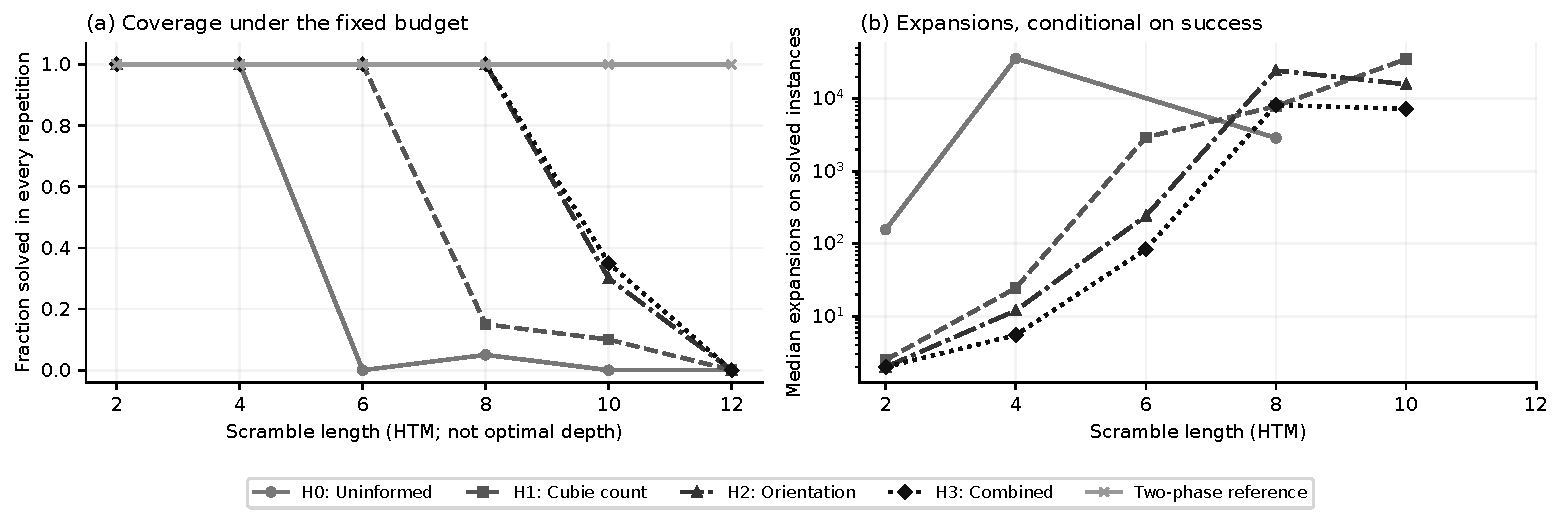
\includegraphics[width=\linewidth]{figures/overview.pdf}
\caption{Measured coverage and search effort. Each length contains twenty distinct states. Right: each method's median is conditional on its own successful subset; missing points indicate no successful instances. The length-eight H0 success is a reminder that scramble length is not optimal distance.}
\label{fig:overview}
\end{figure}

\begin{table}[t]
\centering
\caption{Fixed-corpus summary. Runtime and length medians are conditional on success and therefore compare different subsets. All times are warm search times.}
\label{tab:summary}
\begin{tabular}{lrrr}
\toprule
Method & Solved & Median ms & Median HTM length \\
\midrule
\ResultRows
\bottomrule
\end{tabular}
\end{table}

\paragraph{Coverage improves with stronger bounds.}
Table~\ref{tab:summary} shows H0, H1, H2, and H3 solving \HZeroSolved{}, \HOneSolved{}, \HTwoSolved{}, and \HThreeSolved{} of \InstanceCount{} states, respectively. Both database variants solve every instance through scramble length eight. H2 solves six of twenty length-ten instances; H3 solves seven. Neither reliably solves a length-twelve instance in all repetitions. Across all repetitions, \CustomTimeoutCount{} custom runs hit the time limit; the remaining failures hit the node cap. The large gain from H1 to H2 supports the usefulness of orientation information, while the smaller H2-to-H3 gain shows diminishing coverage returns from this additional abstraction under our budgets.

\paragraph{Fewer expansions do not imply proportional speed.}
On the \PairCount{} common H1/H3 solved states, the median per-instance expansion ratio is \PairNodeRatio{}, but the runtime ratio is approximately \PairTimeRatio{}. On the \CommonCount{} states solved by all custom variants, H1's median is \PairedHOneMs{}\,ms versus \PairedHThreeMs{}\,ms for H3. H3 reduces search work but pays for coordinate ranking and table access. These easy-state timings are small and noisy; the clearest benefit is increased coverage. A next implementation could maintain coordinates incrementally using the existing transition arrays.

\paragraph{The reference trades optimality for reach.}
The two-phase solver solves all 120 states. Among \RefKnown{} states with a proven custom optimum, its default solution matches that optimum in \RefMatches{} cases, with median excess length \RefExcess{} moves. These values describe this particular library configuration on short random walks, not all possible two-phase implementations or tuning strategies. The reference is a useful practical solver but cannot supply ground-truth shortest distances. Its median over all successes also covers harder states than any custom median.

\section{Validation, demonstration, and limitations}
\paragraph{Correctness and reproducibility.}
Every returned sequence is replayed through the custom engine before being accepted. Engine tests compare all face moves and 200 seeded thirty-turn sequences against an independent reference model, and check inverses, invariants, parsing, and facelet conversions. A headless regression solves 36 additional seeded states and checks every solution transition in both engines. All abstract coordinates are checked for rank/unrank correctness and every abstract transition for distance consistency. An exact breadth-first corpus contains all 3,502 states through depth three: admissibility is checked on all, and shortest solutions from all variants on a systematic sample. These tests do not constitute exhaustive full-state verification.

The repository contains the corpus, raw measurements, manifests, aggregation code, vector figures, and reproduction commands. Browser and command-line entry points share the same custom solver. The pixel-style demo provides a complete face net, manual turns, seeded input, cancellation, reversible playback, and a per-move verification log. A replayable tree records the first 240 actual search visits with depths, bounds, and pruning decisions; it is explicitly a partial trace. Trace recording is disabled in timed experiments. Search runs outside the rendering thread; stale worker results are rejected. Camera rotation does not change the state. Reference results are labeled separately and never silently substitute for custom failures.

\paragraph{Limitations.}
The corpus favors states near solved and includes only twenty instances per length; results should not be extrapolated to uniformly random cubes or human scrambling. A single computer and three repetitions provide limited evidence about timing variability. Most failures are node-limited, so our coverage primarily measures search efficiency under that expansion cap. The custom solver has no transposition cache, incremental coordinate updates, symmetry reduction, or larger joint databases. The heuristic ablation isolates changes within our implementation, but the library comparison also changes search strategy and optimization. Neither the library's missing node counts nor initialization costs should be hidden. Team members must understand these boundaries when presenting the results.

\section{Conclusion}
Compact admissible tables substantially extend the range of states our budgeted optimal search can solve. However, a stronger bound has an evaluation cost: measured expansion reductions do not translate directly into runtime improvements. Our implementation makes both effects visible, preserves failures in evaluation, and separates shortest-solution claims from practical reference solving. The most useful next experiment is an incremental-coordinate implementation tested on the same frozen corpus, followed by larger independent state samples.

\clearpage
\begin{thebibliography}{9}
\bibitem[Korf(1997)]{korf}
Richard E. Korf. Finding optimal solutions to Rubik's Cube using pattern databases. In \emph{Proceedings of AAAI}, pages 700--705, 1997.
\bibitem[Kociemba(a)]{coordinates}
Herbert Kociemba. The coordinate level. \url{https://kociemba.org/math/coordlevel.htm}. Accessed November 2026.
\bibitem[Kociemba(b)]{twophase}
Herbert Kociemba. Two-phase algorithm details. \url{https://kociemba.org/math/imptwophase.htm}. Accessed November 2026.
\bibitem{cubejs}
Petri Lehtinen and cubejs contributors. cube.js: JavaScript library for modeling and solving the 3x3x3 Rubik's Cube. Version 1.3.2, MIT license. \url{https://github.com/ldez/cubejs}.
\end{thebibliography}
\end{document}
